\documentclass{standalone}
\usepackage{tikz}
\usetikzlibrary{patterns, positioning}


\begin{document}
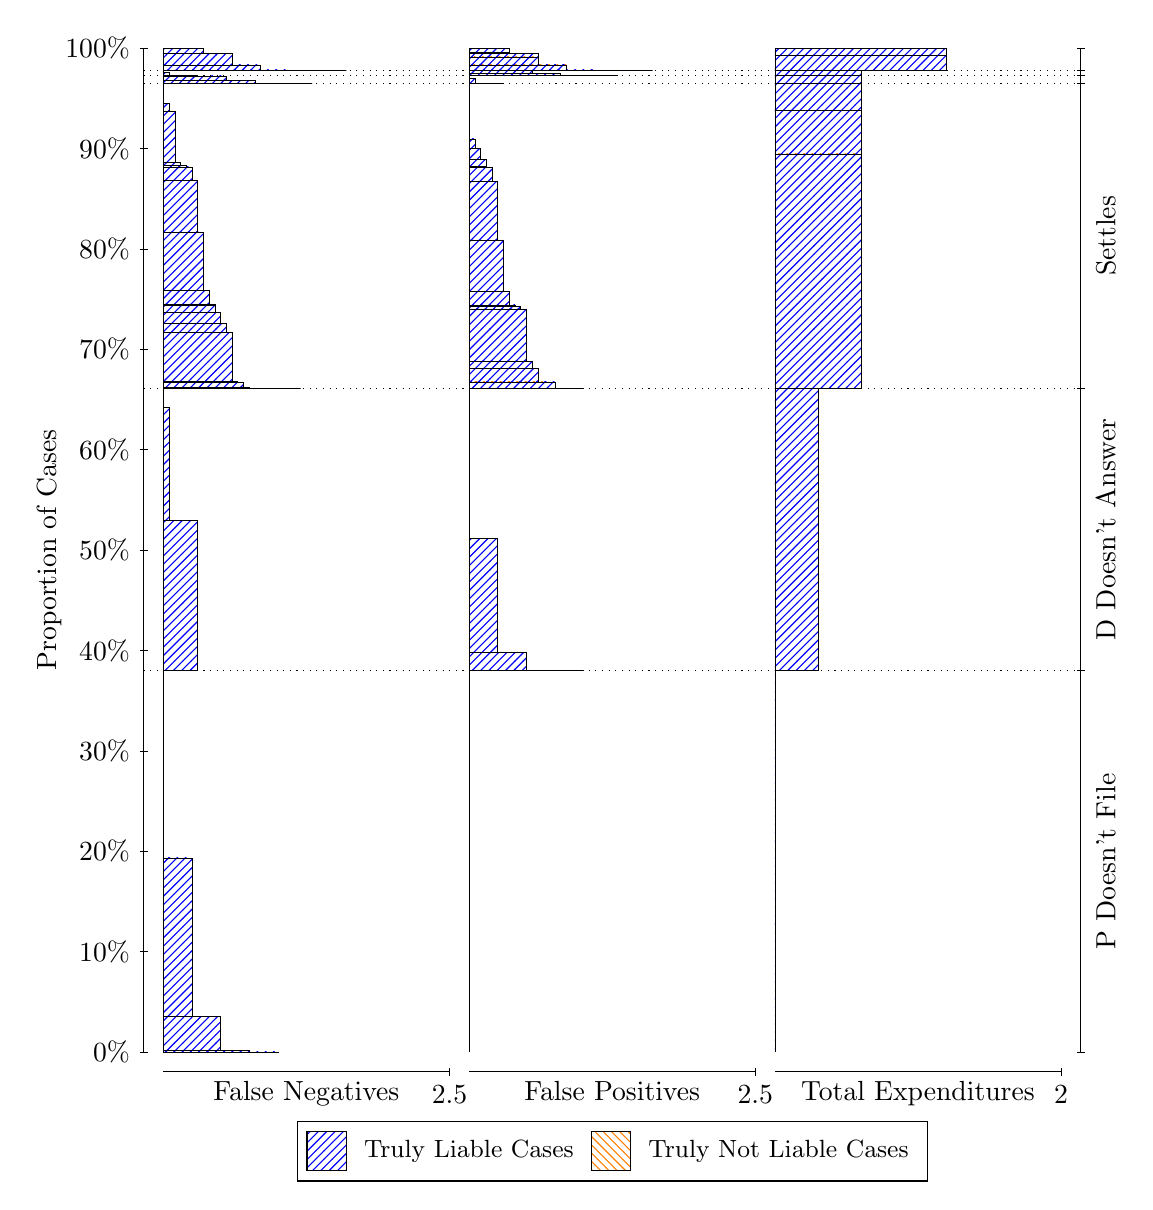
\begin{tikzpicture}
\draw[black, very thin] (1.5,1.75) -- (1.5,14.5);
\node[rotate=90, text=black, anchor=center] at (0.3, 8.125) {Proportion of Cases};
\draw[black, very thin] (1.45,1.75) -- (1.55,1.75);
\node[text=black, anchor=east] at (1.45, 1.75) {0\%};
\draw[black, very thin] (1.45,3.025) -- (1.55,3.025);
\node[text=black, anchor=east] at (1.45, 3.025) {10\%};
\draw[black, very thin] (1.45,4.3) -- (1.55,4.3);
\node[text=black, anchor=east] at (1.45, 4.3) {20\%};
\draw[black, very thin] (1.45,5.575) -- (1.55,5.575);
\node[text=black, anchor=east] at (1.45, 5.575) {30\%};
\draw[black, very thin] (1.45,6.85) -- (1.55,6.85);
\node[text=black, anchor=east] at (1.45, 6.85) {40\%};
\draw[black, very thin] (1.45,8.125) -- (1.55,8.125);
\node[text=black, anchor=east] at (1.45, 8.125) {50\%};
\draw[black, very thin] (1.45,9.4) -- (1.55,9.4);
\node[text=black, anchor=east] at (1.45, 9.4) {60\%};
\draw[black, very thin] (1.45,10.675) -- (1.55,10.675);
\node[text=black, anchor=east] at (1.45, 10.675) {70\%};
\draw[black, very thin] (1.45,11.95) -- (1.55,11.95);
\node[text=black, anchor=east] at (1.45, 11.95) {80\%};
\draw[black, very thin] (1.45,13.225) -- (1.55,13.225);
\node[text=black, anchor=east] at (1.45, 13.225) {90\%};
\draw[black, very thin] (1.45,14.5) -- (1.55,14.5);
\node[text=black, anchor=east] at (1.45, 14.5) {100\%};

\draw[black, very thin] (13.4,1.75) -- (13.4,14.5);
\draw[black, very thin] (13.35,1.75) -- (13.45,1.75);
\node[anchor=west] at (13.35, 1.75) {};
\draw[black, very thin] (13.35,6.5921) -- (13.45,6.5921);
\node[anchor=west] at (13.35, 6.5921) {};
\draw[black, very thin] (13.35,10.177) -- (13.45,10.177);
\node[anchor=west] at (13.35, 10.177) {};
\draw[black, very thin] (13.35,14.053) -- (13.45,14.053);
\node[anchor=west] at (13.35, 14.053) {};
\draw[black, very thin] (13.35,14.148) -- (13.45,14.148);
\node[anchor=west] at (13.35, 14.148) {};
\draw[black, very thin] (13.35,14.216) -- (13.45,14.216);
\node[anchor=west] at (13.35, 14.216) {};
\draw[black, very thin] (13.35,14.5) -- (13.45,14.5);
\node[anchor=west] at (13.35, 14.5) {};

\draw[black, very thin, pattern color=blue, pattern=north east lines] (1.75,1.75) rectangle (3.2033,1.7501);
\draw[black, very thin, pattern color=blue, pattern=north east lines] (1.75,1.7501) rectangle (2.84,1.7664);
\draw[black, very thin, pattern color=blue, pattern=north east lines] (1.75,1.7664) rectangle (2.4767,2.2008);
\draw[black, very thin, pattern color=blue, pattern=north east lines] (1.75,2.2008) rectangle (2.1133,4.2158);
\draw[black, very thin, pattern color=orange, pattern=north west lines] (1.75,4.2158) rectangle (1.75,4.2158);
\draw[black, very thin, pattern color=blue, pattern=north east lines] (1.75,4.2158) rectangle (1.75,6.5921);
\draw[black, very thin, pattern color=blue, pattern=north east lines] (1.75,6.5921) rectangle (2.186,8.4966);
\draw[black, very thin, pattern color=blue, pattern=north east lines] (1.75,8.4966) rectangle (1.8227,9.94);
\draw[black, very thin, pattern color=orange, pattern=north west lines] (1.75,9.94) rectangle (1.75,9.94);
\draw[black, very thin, pattern color=blue, pattern=north east lines] (1.75,9.94) rectangle (1.75,10.177);
\draw[black, very thin, pattern color=blue, pattern=north east lines] (1.75,10.177) rectangle (3.494,10.177);
\draw[black, very thin, pattern color=blue, pattern=north east lines] (1.75,10.177) rectangle (3.2033,10.177);
\draw[black, very thin, pattern color=blue, pattern=north east lines] (1.75,10.177) rectangle (3.1307,10.178);
\draw[black, very thin, pattern color=blue, pattern=north east lines] (1.75,10.178) rectangle (3.058,10.178);
\draw[black, very thin, pattern color=blue, pattern=north east lines] (1.75,10.178) rectangle (2.9127,10.179);
\draw[black, very thin, pattern color=blue, pattern=north east lines] (1.75,10.179) rectangle (2.84,10.195);
\draw[black, very thin, pattern color=blue, pattern=north east lines] (1.75,10.195) rectangle (2.7673,10.254);
\draw[black, very thin, pattern color=blue, pattern=north east lines] (1.75,10.254) rectangle (2.6947,10.263);
\draw[black, very thin, pattern color=blue, pattern=north east lines] (1.75,10.263) rectangle (2.622,10.884);
\draw[black, very thin, pattern color=blue, pattern=north east lines] (1.75,10.884) rectangle (2.5493,11.006);
\draw[black, very thin, pattern color=blue, pattern=north east lines] (1.75,11.006) rectangle (2.4767,11.146);
\draw[black, very thin, pattern color=blue, pattern=north east lines] (1.75,11.146) rectangle (2.404,11.233);
\draw[black, very thin, pattern color=blue, pattern=north east lines] (1.75,11.233) rectangle (2.404,11.246);
\draw[black, very thin, pattern color=blue, pattern=north east lines] (1.75,11.246) rectangle (2.3313,11.423);
\draw[black, very thin, pattern color=blue, pattern=north east lines] (1.75,11.423) rectangle (2.2587,12.166);
\draw[black, very thin, pattern color=blue, pattern=north east lines] (1.75,12.166) rectangle (2.186,12.82);
\draw[black, very thin, pattern color=blue, pattern=north east lines] (1.75,12.82) rectangle (2.1133,12.991);
\draw[black, very thin, pattern color=blue, pattern=north east lines] (1.75,12.991) rectangle (2.0407,13.012);
\draw[black, very thin, pattern color=blue, pattern=north east lines] (1.75,13.012) rectangle (2.0407,13.013);
\draw[black, very thin, pattern color=blue, pattern=north east lines] (1.75,13.013) rectangle (1.968,13.044);
\draw[black, very thin, pattern color=blue, pattern=north east lines] (1.75,13.044) rectangle (1.8953,13.702);
\draw[black, very thin, pattern color=blue, pattern=north east lines] (1.75,13.702) rectangle (1.8227,13.8);
\draw[black, very thin, pattern color=orange, pattern=north west lines] (1.75,13.8) rectangle (1.75,13.8);
\draw[black, very thin, pattern color=blue, pattern=north east lines] (1.75,13.8) rectangle (1.75,14.053);
\draw[black, very thin, pattern color=blue, pattern=north east lines] (1.75,14.053) rectangle (3.6393,14.053);
\draw[black, very thin, pattern color=blue, pattern=north east lines] (1.75,14.053) rectangle (3.276,14.053);
\draw[black, very thin, pattern color=blue, pattern=north east lines] (1.75,14.053) rectangle (2.9127,14.089);
\draw[black, very thin, pattern color=blue, pattern=north east lines] (1.75,14.089) rectangle (2.5493,14.147);
\draw[black, very thin, pattern color=blue, pattern=north east lines] (1.75,14.147) rectangle (2.186,14.148);
\draw[black, very thin, pattern color=orange, pattern=north west lines] (1.75,14.148) rectangle (1.75,14.148);
\draw[black, very thin, pattern color=blue, pattern=north east lines] (1.75,14.148) rectangle (2.186,14.149);
\draw[black, very thin, pattern color=blue, pattern=north east lines] (1.75,14.149) rectangle (1.8227,14.191);
\draw[black, very thin, pattern color=orange, pattern=north west lines] (1.75,14.191) rectangle (1.75,14.191);
\draw[black, very thin, pattern color=blue, pattern=north east lines] (1.75,14.191) rectangle (1.75,14.216);
\draw[black, very thin, pattern color=blue, pattern=north east lines] (1.75,14.216) rectangle (4.0753,14.216);
\draw[black, very thin, pattern color=blue, pattern=north east lines] (1.75,14.216) rectangle (3.712,14.216);
\draw[black, very thin, pattern color=blue, pattern=north east lines] (1.75,14.216) rectangle (3.3487,14.221);
\draw[black, very thin, pattern color=blue, pattern=north east lines] (1.75,14.221) rectangle (2.9853,14.286);
\draw[black, very thin, pattern color=blue, pattern=north east lines] (1.75,14.286) rectangle (2.622,14.429);
\draw[black, very thin, pattern color=blue, pattern=north east lines] (1.75,14.429) rectangle (2.2587,14.495);
\draw[black, very thin, pattern color=blue, pattern=north east lines] (1.75,14.495) rectangle (1.8953,14.5);
\draw[black, very thin, pattern color=orange, pattern=north west lines] (1.75,14.5) rectangle (1.75,14.5);
\draw[black, very thin, pattern color=blue, pattern=north east lines] (1.75,14.5) rectangle (1.75,14.5);
\draw[black, very thin, pattern color=orange, pattern=north west lines] (5.6333,1.75) rectangle (5.6333,1.75);
\draw[black, very thin, pattern color=blue, pattern=north east lines] (5.6333,1.75) rectangle (5.6333,6.5921);
\draw[black, very thin, pattern color=orange, pattern=north west lines] (5.6333,6.5921) rectangle (7.0867,6.5921);
\draw[black, very thin, pattern color=blue, pattern=north east lines] (5.6333,6.5921) rectangle (7.0867,6.5921);
\draw[black, very thin, pattern color=blue, pattern=north east lines] (5.6333,6.5921) rectangle (6.7233,6.5933);
\draw[black, very thin, pattern color=blue, pattern=north east lines] (5.6333,6.5933) rectangle (6.36,6.8289);
\draw[black, very thin, pattern color=blue, pattern=north east lines] (5.6333,6.8289) rectangle (5.9967,8.2722);
\draw[black, very thin, pattern color=blue, pattern=north east lines] (5.6333,8.2722) rectangle (5.6333,10.177);
\draw[black, very thin, pattern color=orange, pattern=north west lines] (5.6333,10.177) rectangle (7.0867,10.177);
\draw[black, very thin, pattern color=blue, pattern=north east lines] (5.6333,10.177) rectangle (7.0867,10.177);
\draw[black, very thin, pattern color=orange, pattern=north west lines] (5.6333,10.177) rectangle (6.9413,10.177);
\draw[black, very thin, pattern color=blue, pattern=north east lines] (5.6333,10.177) rectangle (6.9413,10.177);
\draw[black, very thin, pattern color=orange, pattern=north west lines] (5.6333,10.177) rectangle (6.796,10.177);
\draw[black, very thin, pattern color=blue, pattern=north east lines] (5.6333,10.177) rectangle (6.796,10.177);
\draw[black, very thin, pattern color=blue, pattern=north east lines] (5.6333,10.177) rectangle (6.7233,10.259);
\draw[black, very thin, pattern color=orange, pattern=north west lines] (5.6333,10.259) rectangle (6.6507,10.259);
\draw[black, very thin, pattern color=blue, pattern=north east lines] (5.6333,10.259) rectangle (6.6507,10.26);
\draw[black, very thin, pattern color=blue, pattern=north east lines] (5.6333,10.26) rectangle (6.578,10.26);
\draw[black, very thin, pattern color=orange, pattern=north west lines] (5.6333,10.26) rectangle (6.5053,10.26);
\draw[black, very thin, pattern color=blue, pattern=north east lines] (5.6333,10.26) rectangle (6.5053,10.429);
\draw[black, very thin, pattern color=blue, pattern=north east lines] (5.6333,10.429) rectangle (6.4327,10.528);
\draw[black, very thin, pattern color=blue, pattern=north east lines] (5.6333,10.528) rectangle (6.36,11.186);
\draw[black, very thin, pattern color=blue, pattern=north east lines] (5.6333,11.186) rectangle (6.2873,11.217);
\draw[black, very thin, pattern color=orange, pattern=north west lines] (5.6333,11.217) rectangle (6.2147,11.217);
\draw[black, very thin, pattern color=blue, pattern=north east lines] (5.6333,11.217) rectangle (6.2147,11.217);
\draw[black, very thin, pattern color=blue, pattern=north east lines] (5.6333,11.217) rectangle (6.2147,11.238);
\draw[black, very thin, pattern color=blue, pattern=north east lines] (5.6333,11.238) rectangle (6.142,11.41);
\draw[black, very thin, pattern color=blue, pattern=north east lines] (5.6333,11.41) rectangle (6.0693,12.064);
\draw[black, very thin, pattern color=blue, pattern=north east lines] (5.6333,12.064) rectangle (5.9967,12.807);
\draw[black, very thin, pattern color=blue, pattern=north east lines] (5.6333,12.807) rectangle (5.924,12.984);
\draw[black, very thin, pattern color=blue, pattern=north east lines] (5.6333,12.984) rectangle (5.8513,12.997);
\draw[black, very thin, pattern color=blue, pattern=north east lines] (5.6333,12.997) rectangle (5.8513,13.084);
\draw[black, very thin, pattern color=blue, pattern=north east lines] (5.6333,13.084) rectangle (5.7787,13.223);
\draw[black, very thin, pattern color=blue, pattern=north east lines] (5.6333,13.223) rectangle (5.706,13.346);
\draw[black, very thin, pattern color=blue, pattern=north east lines] (5.6333,13.346) rectangle (5.6333,14.053);
\draw[black, very thin, pattern color=orange, pattern=north west lines] (5.6333,14.053) rectangle (6.0693,14.053);
\draw[black, very thin, pattern color=blue, pattern=north east lines] (5.6333,14.053) rectangle (6.0693,14.054);
\draw[black, very thin, pattern color=blue, pattern=north east lines] (5.6333,14.054) rectangle (5.706,14.113);
\draw[black, very thin, pattern color=blue, pattern=north east lines] (5.6333,14.113) rectangle (5.6333,14.148);
\draw[black, very thin, pattern color=orange, pattern=north west lines] (5.6333,14.148) rectangle (7.5227,14.148);
\draw[black, very thin, pattern color=blue, pattern=north east lines] (5.6333,14.148) rectangle (7.5227,14.148);
\draw[black, very thin, pattern color=blue, pattern=north east lines] (5.6333,14.148) rectangle (7.1593,14.148);
\draw[black, very thin, pattern color=blue, pattern=north east lines] (5.6333,14.148) rectangle (6.796,14.174);
\draw[black, very thin, pattern color=blue, pattern=north east lines] (5.6333,14.174) rectangle (6.4327,14.215);
\draw[black, very thin, pattern color=blue, pattern=north east lines] (5.6333,14.215) rectangle (6.0693,14.216);
\draw[black, very thin, pattern color=orange, pattern=north west lines] (5.6333,14.216) rectangle (7.9587,14.216);
\draw[black, very thin, pattern color=blue, pattern=north east lines] (5.6333,14.216) rectangle (7.9587,14.216);
\draw[black, very thin, pattern color=orange, pattern=north west lines] (5.6333,14.216) rectangle (7.5953,14.216);
\draw[black, very thin, pattern color=blue, pattern=north east lines] (5.6333,14.216) rectangle (7.5953,14.216);
\draw[black, very thin, pattern color=orange, pattern=north west lines] (5.6333,14.216) rectangle (7.232,14.216);
\draw[black, very thin, pattern color=blue, pattern=north east lines] (5.6333,14.216) rectangle (7.232,14.221);
\draw[black, very thin, pattern color=blue, pattern=north east lines] (5.6333,14.221) rectangle (6.8687,14.286);
\draw[black, very thin, pattern color=orange, pattern=north west lines] (5.6333,14.286) rectangle (6.8687,14.286);
\draw[black, very thin, pattern color=blue, pattern=north east lines] (5.6333,14.286) rectangle (6.8687,14.287);
\draw[black, very thin, pattern color=blue, pattern=north east lines] (5.6333,14.287) rectangle (6.5053,14.388);
\draw[black, very thin, pattern color=orange, pattern=north west lines] (5.6333,14.388) rectangle (6.5053,14.388);
\draw[black, very thin, pattern color=blue, pattern=north east lines] (5.6333,14.388) rectangle (6.5053,14.43);
\draw[black, very thin, pattern color=blue, pattern=north east lines] (5.6333,14.43) rectangle (6.142,14.447);
\draw[black, very thin, pattern color=blue, pattern=north east lines] (5.6333,14.447) rectangle (6.142,14.495);
\draw[black, very thin, pattern color=blue, pattern=north east lines] (5.6333,14.495) rectangle (5.7787,14.495);
\draw[black, very thin, pattern color=blue, pattern=north east lines] (5.6333,14.495) rectangle (5.7787,14.5);
\draw[black, very thin, pattern color=blue, pattern=north east lines] (5.6333,14.5) rectangle (5.6333,14.5);
\draw[black, very thin, pattern color=orange, pattern=north west lines] (9.5167,1.75) rectangle (9.5167,1.75);
\draw[black, very thin, pattern color=blue, pattern=north east lines] (9.5167,1.75) rectangle (9.5167,6.5921);
\draw[black, very thin, pattern color=orange, pattern=north west lines] (9.5167,6.5921) rectangle (10.062,6.5921);
\draw[black, very thin, pattern color=blue, pattern=north east lines] (9.5167,6.5921) rectangle (10.062,10.177);
\draw[black, very thin, pattern color=orange, pattern=north west lines] (9.5167,10.177) rectangle (10.607,10.177);
\draw[black, very thin, pattern color=blue, pattern=north east lines] (9.5167,10.177) rectangle (10.607,13.157);
\draw[black, very thin, pattern color=orange, pattern=north west lines] (9.5167,13.157) rectangle (10.607,13.157);
\draw[black, very thin, pattern color=blue, pattern=north east lines] (9.5167,13.157) rectangle (10.607,13.707);
\draw[black, very thin, pattern color=orange, pattern=north west lines] (9.5167,13.707) rectangle (10.607,13.707);
\draw[black, very thin, pattern color=blue, pattern=north east lines] (9.5167,13.707) rectangle (10.607,14.053);
\draw[black, very thin, pattern color=orange, pattern=north west lines] (9.5167,14.053) rectangle (10.607,14.053);
\draw[black, very thin, pattern color=blue, pattern=north east lines] (9.5167,14.053) rectangle (10.607,14.148);
\draw[black, very thin, pattern color=orange, pattern=north west lines] (9.5167,14.148) rectangle (10.607,14.148);
\draw[black, very thin, pattern color=blue, pattern=north east lines] (9.5167,14.148) rectangle (10.607,14.216);
\draw[black, very thin, pattern color=orange, pattern=north west lines] (9.5167,14.216) rectangle (11.697,14.216);
\draw[black, very thin, pattern color=blue, pattern=north east lines] (9.5167,14.216) rectangle (11.697,14.405);
\draw[black, very thin, pattern color=orange, pattern=north west lines] (9.5167,14.405) rectangle (11.697,14.405);
\draw[black, very thin, pattern color=blue, pattern=north east lines] (9.5167,14.405) rectangle (11.697,14.5);
\draw[black, dotted] (1.5,6.5921) -- (13.4,6.5921);
\draw[black, dotted] (1.5,10.177) -- (13.4,10.177);
\draw[black, dotted] (1.5,14.053) -- (13.4,14.053);
\draw[black, dotted] (1.5,14.148) -- (13.4,14.148);
\draw[black, dotted] (1.5,14.216) -- (13.4,14.216);
\draw[black, very thin] (1.75,1.5) -- (5.3833,1.5);
\node[text=black, anchor=north] at (3.5667, 1.5) {False Negatives};
\draw[black, very thin] (5.3833,1.45) -- (5.3833,1.55);
\node[text=black, anchor=north] at (5.3833, 1.45) {2.5};

\draw[black, very thin] (5.6333,1.5) -- (9.2667,1.5);
\node[text=black, anchor=north] at (7.45, 1.5) {False Positives};
\draw[black, very thin] (9.2667,1.45) -- (9.2667,1.55);
\node[text=black, anchor=north] at (9.2667, 1.45) {2.5};

\draw[black, very thin] (9.5167,1.5) -- (13.15,1.5);
\node[text=black, anchor=north] at (11.333, 1.5) {Total Expenditures};
\draw[black, very thin] (13.15,1.45) -- (13.15,1.55);
\node[text=black, anchor=north] at (13.15, 1.45) {2};

\node[text=black, centered, rotate=90] at (13.72, 4.171) {P Doesn't File};
\node[text=black, centered, rotate=90] at (13.72, 8.3844) {D Doesn't Answer};
\node[text=black, centered, rotate=90] at (13.72, 12.115) {Settles};




\draw (7.449999999999999,1.5) node[draw=none] (baseCoordinate) {};
\begin{scope}[align=center]
        \matrix[scale=0.5, draw=black, below=0.5cm of baseCoordinate, nodes={draw}, column sep=0.1cm]{
            \node[rectangle, draw, minimum width=0.5cm, minimum height=0.5cm, pattern color=blue, pattern=north east lines] {}; &
            \node[draw=none, font=\small, text=black] (B) {Truly Liable Cases}; &
            \node[rectangle, draw, minimum width=0.5cm, minimum height=0.5cm, pattern color=orange, pattern=north west lines] {}; &
            \node[draw=none, font=\small, text=black] (B) {Truly Not Liable Cases}; \\
            };
\end{scope}

\end{tikzpicture}
\end{document}